\section{Methods}
\label{sec:methods}

\begin{figure}[htbp]
  \centering
  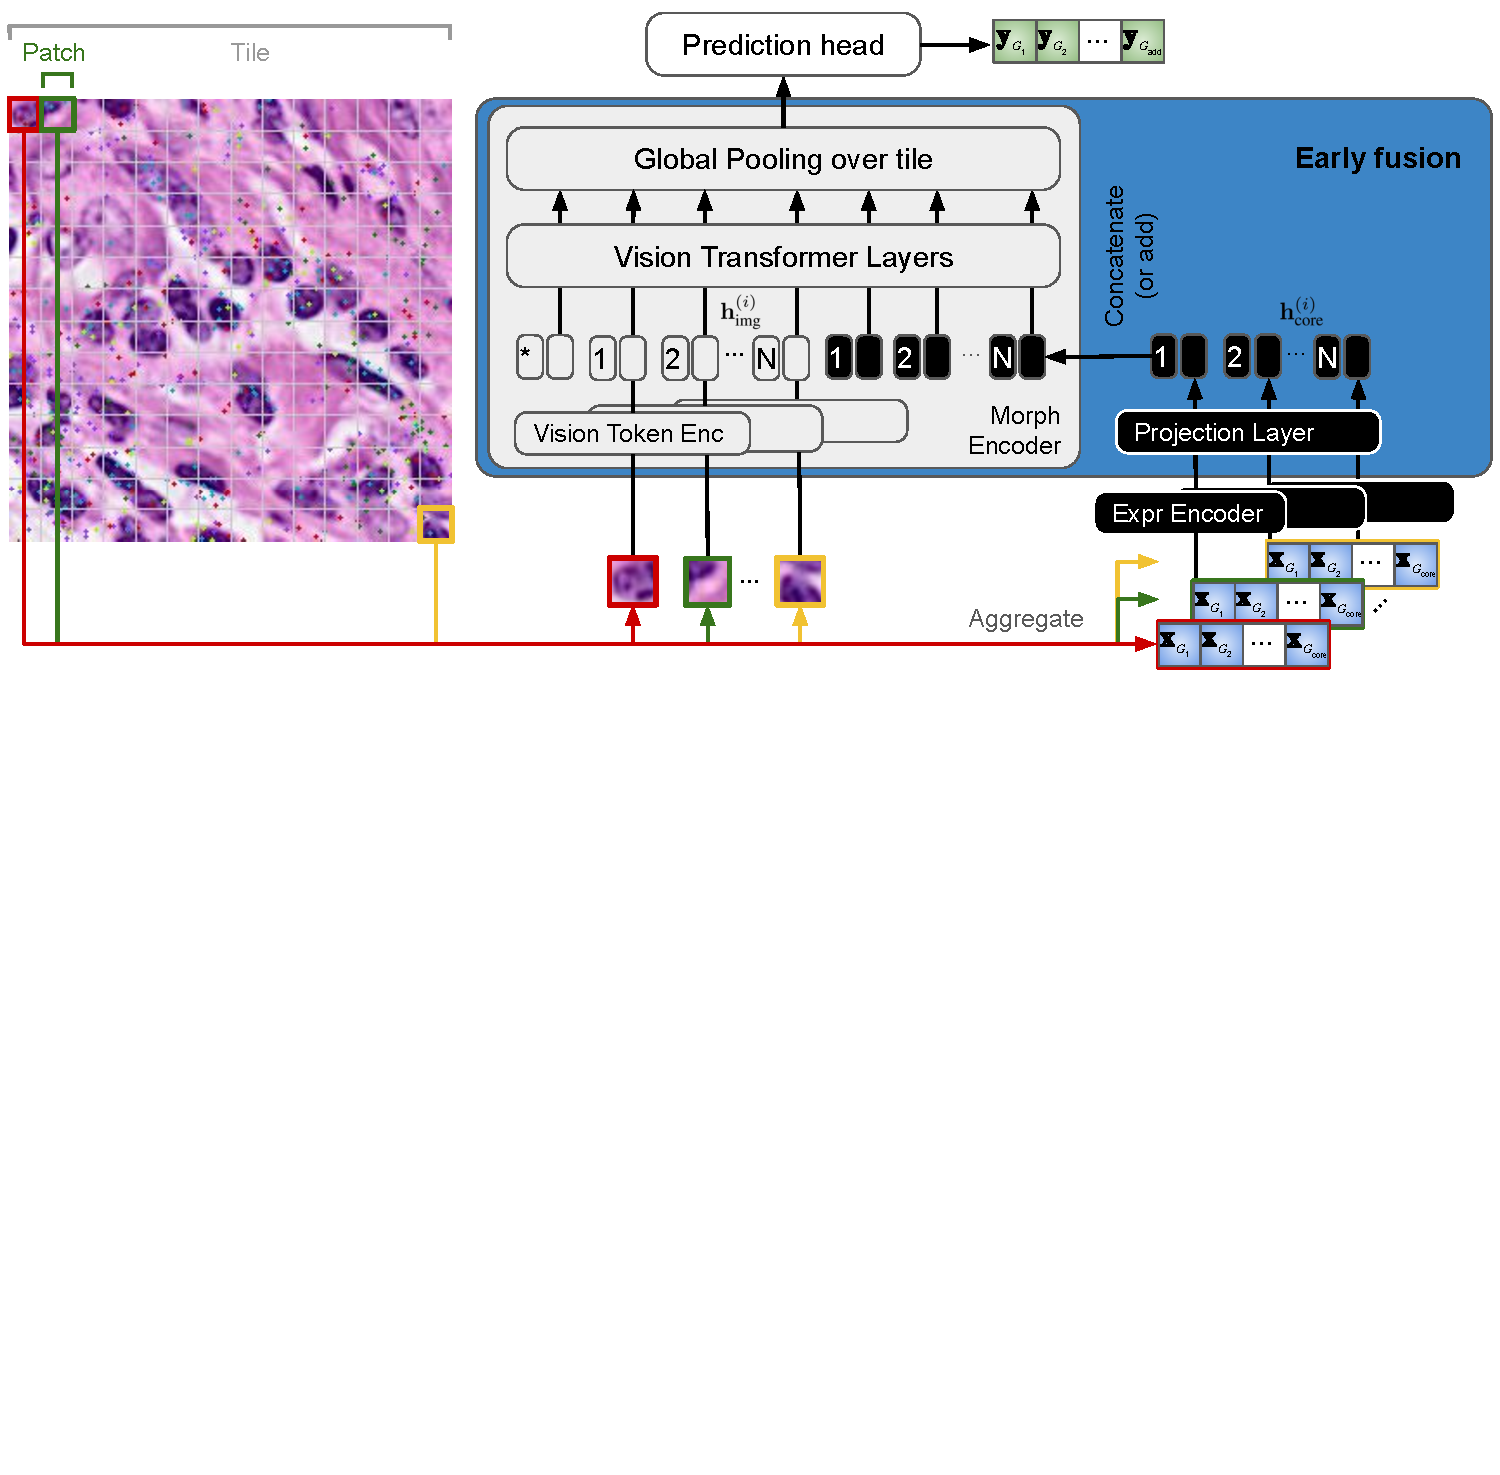
\includegraphics[width=\textwidth]{figures/model_overview.pdf}
\caption{\textbf{Model architecture for multimodal prediction of spatial gene expression and cell type composition.}
\textit{Left:} A representative $512 \times 512$ pixel tile cropped from a whole-slide H\&E image, overlaid with the Vision Transformer (ViT) patch grid. Each grid cell corresponds to a $16 \times 16$ pixel image patch that is encoded as a single token. Coloured crosses mark a subset of spatially aligned Xenium transcripts, demonstrating the co-localisation of transcriptomic measurements with the ViT token grid.
\textit{Right:} The multimodal model processes two aligned token sequences. Image patches are embedded by the \emph{Morph Encoder} into a sequence of morphological token embeddings $\mathbf{h}_{\mathrm{img}}^{(i)}$. In parallel, transcripts aggregated within each ViT patch position are encoded by the \emph{Expr Encoder} and projected to the same embedding dimensionality, yielding a spatially aligned sequence of transcriptomic token embeddings $\mathbf{h}_{\mathrm{core}}^{(i)}$. The two token sequences are fused by either concatenation or element-wise addition (\emph{early fusion}), and a learnable classification token (\texttt{[CLS]}) is prepended to the combined sequence. The resulting sequence is processed by the remaining ViT transformer layers, which allow all tokens to interact via self-attention. The \texttt{[CLS]} token aggregates information across both modalities and spatial positions into a single tile-level representation, which is passed to a linear prediction head to predict either add-on panel gene expression or cell type abundances.}
  \label{fig:p-fus:architecture}
\end{figure}

In this section, we describe our approach for predicting spatial gene expression and cell type composition from histopathology images and partial transcriptomic data. We detail our data processing pipeline, formalize the two prediction tasks, present the model architectures, and describe our training and evaluation protocols.

\paragraph{Terminology.}
Throughout this paper we use the following terms consistently. A \emph{whole-slide image} (WSI) refers to a high-resolution digital scan of a histological tissue section, typically captured at $0.25$--$0.5\,\mu\text{m}$ per pixel. A \emph{tile} is a fixed-size, spatially localized crop of the WSI; we work with $512 \times 512$ pixel tiles at $0.5\,\mu\text{m}/\text{px}$, corresponding to a $256 \times 256\,\mu\text{m}$ tissue area. Within the ViT architecture, each tile is further divided into a regular grid of non-overlapping $16 \times 16$ pixel sub-regions called \emph{patches}. Each patch is mapped to a \emph{token}, a $d$-dimensional vector that is the fundamental unit of computation in the transformer. Transcript and morphology features are both represented as token sequences, with one token per ViT patch position, enabling direct spatial alignment between the two modalities.

\paragraph{Model naming.}
We use the following names consistently throughout the paper:
\begin{itemize}
  \item \textbf{vision}: morphology-only ViT trained end-to-end; the primary variant uses ViT-S, with ViT-B evaluated as a capacity ablation.
  \item \textbf{CONCH}: frozen H\&E foundation model baseline~\cite{lu_multimodalgenerativeai_2024}, evaluated as a representative pretrained vision encoder.
  \item \textbf{expr-tile}: expression-only model with tile-level transcript aggregation.
  \item \textbf{expr-token}: expression-only model with token-level transcript aggregation.
  \item \textbf{Geneformer}: frozen expression foundation model baseline~\cite{theodoris_transferlearningenables_2023}.
  \item \textbf{early-fusion-add} / \textbf{early-fusion-concat}: early fusion with element-wise addition or concatenation of transcript tokens into the ViT stream.
  \item \textbf{late-fusion-tile-add} / \textbf{late-fusion-tile-concat}: late fusion with tile-level transcript embeddings combined by addition or concatenation.
  \item \textbf{late-fusion-token-add} / \textbf{late-fusion-token-concat}: late fusion with token-level (pooled) transcript embeddings combined by addition or concatenation.
\end{itemize}

\subsection*{Data Processing}
\label{sec:data-processing}

\subsubsection{H\&E and Xenium Spatial Alignment}
\label{sec:he-and-xenium-spatial-alignment}

We register the H\&E whole-slide image (WSI) to the Xenium coordinate system using the DAPI channel and manually selected landmark correspondences. These landmarks are used to estimate an affine transformation that maps Xenium transcript coordinates into H\&E pixel space. To account for local tissue deformations, we partition each tissue section into regions and estimate a separate affine transform per region if necessary. Finally, we crop the WSI to the transcript-containing area to restrict downstream tiling to regions with Xenium measurements.

We tile each WSI into $512\times512$ pixel tiles with a stride of 256 pixels at a resolution of $0.5\,\mu$m per pixel. The 50\% overlap ensures that tissue structures near tile boundaries are captured across multiple tiles, reducing information loss from cells split at edges. Each tile is resized to $224\times224$ pixels prior to inference, after which the vision transformer tokenizes it into $16\times16$ pixel patches. At the resulting effective resolution of approximately $1.14\,\mu$m per pixel, each patch spans roughly $18\,\mu$m, approximately the diameter of a human lung cell~\cite{crapo_cellnumbercell_1982}.

To ensure sufficient signal for downstream modeling, we apply task-specific quality filters. For gene expression prediction, we filter tiles to contain at least 1,000 transcripts. For cell type count prediction, we filter tiles to contain at least 20 cells. Cell density per tile does not correlate with whole-slide image size, supporting the validity of cross-sample comparisons.

\subsubsection{Cell Phenotyping}
\label{sec:p-fus:cell-phenotyping}

Cell type annotations were provided by collaborators at the Biomedical Data Science Center at CHUV (Daria Buszta, Jonathan Bac, and Senbai Kang) using a reference-based deconvolution approach. Matched single-nucleus RNA-seq (snRNA-seq) data were generated from FFPE tissue sections adjacent to those used for Xenium profiling, processed with CellRanger and Seurat~\cite{bilous_transcriptscellsdissecting_2025}. Cell type labels were transferred to Xenium profiles using Robust Cell Type Decomposition (RCTD)~\cite{cable_robustdecompositioncell_2022} in doublet mode. Cells with fewer than 10 transcripts or 5 detected genes were excluded; annotation was performed per sample, with malignant cell references restricted to donor-matched profiles where available.

\subsubsection{Datasets}
\label{sec:datasets}

\paragraph{BEAT.}
Our primary dataset is an internal cancer cohort comprising 159 patients with paired H\&E histology and Xenium spatial transcriptomics measurements. The Xenium panel includes the core Human Immuno-Oncology Panel ($G_{\text{core}} = 380$ genes) and a custom add-on panel ($G_{\text{add}} = 100$ genes) selected for relevance to cancer biology and treatment response. Of the 159 patients, 153 have cell type annotations derived as described above. The dataset provides a challenging and realistic testbed reflecting the complexity and heterogeneity of tumor microenvironments.

\paragraph{HEST1k.}
We additionally evaluate on HEST-1k~\cite{jaume_hest1kdatasetspatial_2024}, a large-scale public compendium of paired H\&E and spatial transcriptomics data spanning diverse tissues and platforms. Samples are preprocessed following the standard HEST pipeline and evaluated using HVG-50 as prediction targets. The broad tissue diversity tests cross-dataset generalization of all model variants.

\paragraph{HESCAPE.}
HESCAPE~\cite{gindra_largescalebenchmarkcrossmodal_2025} defines a curated benchmark subset of HEST1k samples with a standardized gene panel. We use HESCAPE both as a dataset and as a panel definition; experiments on this subset allow direct comparison to prior cross-modal representation learning benchmarks.

\subsection*{Problem Formulation}
\label{sec:problem-formulation}

\paragraph{Gene Expression Prediction.}
For each tile, our objective is to predict the add-on gene expression vector $\mathbf{y}\in\mathbb{R}^{G_{\text{add}}}$ given H\&E histology and/or transcripts from the core gene panel. We aggregate all transcripts within each tile's spatial boundaries and apply a log$_{1+}$p transformation. We evaluate two target panel configurations: the 50 most highly variable genes (HVG-50) and the HESCAPE panel genes.

\paragraph{Cell Type Count Prediction.}
For each tile, we predict a vector $\mathbf{c}\in\mathbb{R}^{39}$ representing the log$_{1+}$p-transformed counts of 39 cell types across the cohort. This task complements gene expression prediction by requiring models to capture cellular phenotypes and their spatial distributions from histological and transcriptomic features.

\subsection*{Model Architecture}
\label{sec:model-architecture}

Our architecture integrates visual and transcriptomic modalities through a ViT backbone that processes spatially aligned tokens from both data types.

\subsubsection{Image Encoding}
\label{sec:image-encoding}

Each H\&E tile is resized from $512\times512$ to $224\times224$ pixels and processed by the vision token encoder component of a ViT, which we refer to as the \emph{Morph Encoder}. This yields $N$ patch token embeddings plus a classification (CLS) token: $\mathbf{H}_{\text{img}}\in\mathbb{R}^{(N+1)\times d}$, where $d$ is the embedding dimension.

\subsubsection{Transcript Encoding}
\label{sec:transcript-encoding}

We explore two transcript representation strategies:

\textbf{Tile-level aggregation.} All core panel transcripts within a tile are aggregated into a single vector $\mathbf{x}_{\text{core}}\in\mathbb{R}^{G_{\text{core}}}$, discarding within-tile spatial heterogeneity.

\textbf{Token-level aggregation.} Transcripts are aggregated at the resolution of individual ViT patch positions, yielding a spatially aligned sequence $\{\mathbf{x}_{\text{core}}^{(i)}\}_{i=1}^{N}$. Each token is encoded by a learned MLP projection $f_{\boldsymbol{\theta}}$:
\begin{equation}
    \mathbf{h}_{\text{core}}^{(i)} = f_{\boldsymbol{\theta}}\!\left(\mathbf{x}_{\text{core}}^{(i)}\right),
\end{equation}
where $f_{\boldsymbol{\theta}} : \mathbb{R}^{G_{\text{core}}} \to \mathbb{R}^{d}$ constitutes our \emph{Expr Encoder}.

\subsection*{Unimodal Baselines}
\label{sec:baseline-methods}

\subsubsection{Vision Models}
\label{sec:vision-models}

The \textbf{vision} model is a ViT fine-tuned end-to-end on the target task. The primary configuration uses ViT-S; ViT-B is evaluated as part of the capacity ablation. \textbf{CONCH}~\cite{lu_multimodalgenerativeai_2024} is a visual-language foundation model pretrained on diverse histopathology images and biomedical text, used as a frozen feature extractor with a task-specific linear head. We additionally report results for Phikon~\cite{filiot_phikonv2largepublic_2024} and the OmiCLIP/Loki image encoder~\cite{chen_visualomicsfoundation_2025} in the appendix.

\subsubsection{Expression Models}
\label{sec:expression-models}

\textbf{expr-tile} and \textbf{expr-token} are transcript-only models that predict targets from core panel measurements using tile-level and token-level transcript aggregation, respectively; for \textbf{expr-token}, the token embeddings are globally averaged before the prediction head. \textbf{Geneformer}~\cite{theodoris_transferlearningenables_2023} (\texttt{gf-12L-38M-i4096} checkpoint, 12 layers, 38M parameters) is used as a frozen expression foundation model baseline.

\subsubsection{Minimum-MAE Baseline}
\label{sec:minimum-mae-baseline}

For each target gene $t$, this baseline identifies the single core gene that best predicts $t$ on the training set by MAE:
\begin{equation}
s^{\ast}(t)=\arg\min_{s\in G_{\text{core}}}\mathrm{MAE}\!\left(y_{\cdot,t},x_{\cdot,s}\right).
\end{equation}
The prediction is the direct expression value of $s^{*}(t)$. This baseline quantifies how much can be explained by simple cross-panel gene--gene correlations.

\subsection*{Multimodal Fusion Strategies}
\label{sec:multimodal-fusion-strategies}

\subsubsection{Early Fusion}
\label{sec:early-fusion}

Early fusion integrates transcript tokens directly into the ViT token stream before any transformer processing. Given image embeddings $\mathbf{H}_{\text{img}}\in\mathbb{R}^{(N+1)\times d}$ and token-level transcript embeddings $\mathbf{H}_{\text{core}}\in\mathbb{R}^{N\times d}$:

\begin{itemize}
\item \textbf{early-fusion-add}: $\mathbf{h}_{\text{fused}}^{(i)} = \mathbf{h}_{\text{img}}^{(i)} + \mathbf{h}_{\text{core}}^{(i)}$ for each spatial position $i$; the CLS token is unchanged.
\item \textbf{early-fusion-concat}: image and transcript token sequences are concatenated along the sequence dimension, yielding a combined sequence of length $2N+1$.
\end{itemize}

The fused sequence is processed by the remaining ViT layers via self-attention, and a linear head maps the CLS token to predictions.

\subsubsection{Late Fusion}
\label{sec:late-fusion}

In late fusion, each modality is encoded independently and the resulting embeddings are combined at the embedding level. Let $\mathbf{z}_{\text{img}}\in\mathbb{R}^{d}$ be the image CLS embedding and $\mathbf{z}_{\text{core}}\in\mathbb{R}^{d}$ be a pooled transcript embedding.

\begin{itemize}
\item \textbf{late-fusion-tile-add} / \textbf{late-fusion-tile-concat}: tile-level transcript aggregation; combined by addition or concatenation.
\item \textbf{late-fusion-token-add} / \textbf{late-fusion-token-concat}: token-level transcript aggregation (mean-pooled); combined by addition or concatenation.
\end{itemize}

Comparing tile- and token-level late fusion isolates whether preserving within-tile spatial structure during encoding improves predictive performance, even when spatial information is discarded before the prediction head.

\paragraph{Encoder capacity.}
We evaluate two capacity levels applied consistently across all models:
\begin{itemize}
  \item \textbf{Low capacity}: ViT-S backbone; 1-layer \emph{Expr Encoder} MLP.
  \item \textbf{High capacity}: ViT-B backbone; 2-layer \emph{Expr Encoder} MLP of 128 hidden units per layer with ReLU activations.
\end{itemize}

\subsection*{Contrastive Pretraining}
\label{sec:contrastive-pretraining}

To further investigate token-level versus tile-level transcript representations, we conduct CLIP-style contrastive pretraining~\cite{radford_learningtransferablevisual_2021}. Given a batch of $B$ paired tiles, let $\mathbf{z}_{\text{img}}^{(i)}$ and $\mathbf{z}_{\text{core}}^{(i)}$ be $\ell_2$-normalized image and transcript embeddings. The symmetric InfoNCE loss is:
\begin{equation}
  \mathcal{L}_{\text{CLIP}} = -\frac{1}{2B}\sum_{i=1}^{B}\left[
    \log \frac{e^{S_{ii}/\tau}}{\sum_{j} e^{S_{ij}/\tau}}
    +
    \log \frac{e^{S_{ii}/\tau}}{\sum_{j} e^{S_{ji}/\tau}}
  \right],
  \label{eq:clip-loss}
\end{equation}
where $S_{ij} = {\mathbf{z}_{\text{img}}^{(i)}}^\top \mathbf{z}_{\text{core}}^{(j)}$ and $\tau>0$ is a learnable temperature. We compare \textbf{CLIP-tile} (tile-aggregated transcript embedding) against \textbf{CLIP-token} (mean-pooled token-level embeddings).

\subsection*{Downstream Clinical Evaluation via MIL}
\label{sec:mil-evaluation}

To assess the clinical utility of the learned representations, we extract tile-level embeddings from each model variant and train multiple-instance learning (MIL) aggregators on two tasks: (i)~\textbf{histology classification} and (ii)~\textbf{survival prediction}. We use an attention-based MIL (ABMIL) aggregator~\cite{ilse_attentionbaseddeeplearning_2018} with fixed, frozen tile embeddings, so that differences in downstream performance directly reflect the quality of the learned representations. Experiments are conducted on the BEAT cohort and extended to HEST1k and HESCAPE where labels are available.

\subsection*{Training and Evaluation}
\label{sec:training-and-evaluation}

\subsubsection{Loss Function}
\label{sec:loss-function}

All models are trained with mean squared error (MSE):
\begin{equation}
\mathcal{L} = \frac{1}{G}\sum_{g=1}^{G} (\hat{y}_g - y_g)^2,
\end{equation}
where $G$ is the number of target genes or cell types.

\subsubsection{Training Protocol}
\label{sec:training-protocol}

Models were implemented in PyTorch and PyTorch Lightning. Training was performed on NVIDIA A100 GPUs (40\,GB) using mixed-precision (FP16). Each configuration was trained for up to 35 epochs with early stopping on validation performance. We used AdamW with a differential learning rate ($10^{-4}$ for the prediction head, $10^{-5}$ for backbone parameters), weight decay $10^{-3}$, global batch size 256--512, gradient clipping to norm 1.0, and a cosine learning rate schedule with 5-epoch linear warmup.

Data were split into training, validation, and test partitions at the patient level. Details are provided in \autoref{tab:p-fus:cohort}.

\subsubsection{Evaluation Metrics}
\label{sec:evaluation-metrics}

Following prior work~\cite{chen_visualomicsfoundation_2025,gindra_largescalebenchmarkcrossmodal_2025}, we report per-gene (or per-cell-type) metrics averaged across all targets:
\begin{itemize}
\item \textbf{Pearson correlation (PCC)}: linear relationship between predicted and true values across tiles.
\item \textbf{Spearman correlation (SCC)}: rank-based correlation, robust to non-linear transformations.
\item \textbf{MSE}: average squared deviation between predictions and ground truth.
\end{itemize}

Because samples differ widely in tile count, tile-weighted averages may be dominated by large WSIs. We therefore additionally report an \textbf{equal-weighted sample-level score}: we compute the metric for each sample independently (aggregating its tiles) and average uniformly across samples. This score reflects per-patient predictive performance and is complementary to tile-level metrics.
